\documentclass{report}
\usepackage[T1]{fontenc} % Fontes T1
\usepackage[utf8]{inputenc} % Input UTF8
\usepackage[backend=biber, style=ieee]{biblatex} % para usar bibliografia
\usepackage{csquotes}
\usepackage[portuguese]{babel} %Usar língua portuguesa
\usepackage{blindtext} % Gerar texto automaticamente
\usepackage[printonlyused]{acronym}
\usepackage{hyperref} % para autoref
\usepackage{graphicx}
\usepackage{indentfirst}
\usepackage{float}


\bibliography{bibliografia}


\begin{document}
%%
% Definições
%
\def\titulo{Alterações Climáticas}
\def\data{11/11/2023}
\def\autores{Catarina Monteiro Rabaça, Rita Pipa Godinho}
\def\autorescontactos{(119582) catarina.rabaca@ua.pt, (119875) rita.godinho@ua.pt}
\def\versao{1.0}
\def\departamento{Dept. de Eletrónica, Telecomunicações e Informática}
\def\empresa{Universidade de Aveiro}
\def\logotipo{ua.pdf}
%
%%%%%% CAPA %%%%%%
%
\begin{titlepage}

\begin{center}
%
\vspace*{50mm}
%
{\Huge \titulo}\\ 
%
\vspace{10mm}
%
{\Large \empresa}\\
%
\vspace{10mm}
%
{\LARGE \autores}\\ 
%
\vspace{30mm}
%
\begin{figure}[h]
\center
\includegraphics{\logotipo}
\end{figure}
%
\vspace{30mm}
\end{center}
%
\begin{flushright}
\versao
\end{flushright}
\end{titlepage}

%%  Página de Título %%
\title{%
{\Huge\textbf{\titulo}}\\
{\Large \departamento\\ \empresa}
}
%
\author{%
    \autores \\
    \autorescontactos
}
%
\date{\today}
%
\maketitle

\pagenumbering{roman}

%%%%%% RESUMO %%%%%%
\begin{abstract}
	
Neste projeto, exploraremos a problemática das alterações climáticas, um tema que suscita crescente preocupação devido aos seus impactos expressivos nos âmbitos ecológico, social e económico.

Destacaremos a importância de compreender e minimizar tais impactos, além de ressaltar a necessidade premente de uma ação coletiva em escala internacional.

A metodologia adotada nesta pesquisa fundamenta-se em uma abordagem multidisciplinar que integra dados climáticos, analisando as relações entre passado, atualidade e futuro no que concerne à evolução desta problemática.

Utilizaremos fontes confiáveis, como relatórios científicos e dados de organizações renomadas no campo das alterações climáticas, para assegurar a precisão das nossas conclusões. 

\textbf{TODAS} as fontes serão minuciosamente descritas e devidamente referenciadas na bibliografia.

Identificaremos áreas particularmente vulneráveis e os setores socioeconómicos mais impactados. Enfatizaremos a relevância da educação ambiental e da implementação de políticas sustentáveis como meios cruciais para mitigar esses impactos.

As nossas conclusões sublinham a urgência de adotar medidas para reduzir as emissões de gases com efeito de estufa, promover práticas sustentáveis e adaptar as infraestruturas às inevitáveis alterações climáticas.

Este estudo contribuirá para uma compreensão mais aprofundada das alterações climáticas e fornecerá uma base sólida para a elaboração de políticas e práticas visando a construção de um futuro mais sustentável e resiliente.
\end{abstract}

%%%%%% Agradecimentos %%%%%%
% Segundo glisc deveria aparecer após conclusão...
%\renewcommand{\abstractname}{Agradecimentos}
%\begin{abstract}
%	Eventuais agradecimentos.
%	Comentar bloco caso não existam agradecimentos a fazer.
%\end{abstract}

\renewcommand{\contentsname}{Índice}
\tableofcontents
% \listoftables     % descomentar se necessário
% \listoffigures    % descomentar se necessário


%%%%%%%%%%%%%%%%%%%%%%%%%%%%%%%
\clearpage
\pagenumbering{arabic}


%%%%%%%%%%%%%%%%%%%%%%%%%%%%%%%%
\chapter{Introdução}
\label{chap.introducao}

As \ac{ac} têm imergido como um desafio cada vez maior para a sociedade, já que os impactos das mesmas, são cada vez mais presentes na atualidade.

O facto da maioria dos fatores que impulsionam as mesmas derivarem da mão humana, faz com que este tópico seja ainda mais discutível e alarmante, visto que todo o sistema terrestre, ( composto pela atmosfera, biosfera, geosfera e hidrosfera), está a sofrer alterações que em muitos casos se encontram em níveis irreversíveis.

Ao longo do documento irá ser possível identificar 3 capítulos principais:

\textbf{Desmistificando as alterações climáticas}, onde abordaremos o contexto histórico das \ac{ac}, fazendo referência também ao estado atual e ao possível estado futuro do globo.

\textbf{Contribuintes}, onde serão expostos os principais colaboradores para o aumento drástico das \ac{ac}, especificando de maneira clara cada um deles.

\textbf{Combate}, capítulo onde serão expostas as principais medidas para combater as \ac{ac}

Na conclusão apresentaremos então de maneira sintetizada ao objetivo principal do projeto assim como analisar todos os tópicos abordados durante a tese. 

Dessa forma, este relatório destina-se a compreender melhor o que são as \ac{ac}, os impactos que as mesmas estão a ter sobre o planeta, como conseguir amenizar a maioria dos danos já provocados por elas e como enfrentar possíveis problemas que estas perturbações possam causar futuramente. 



\chapter{Desmistificando as Alterações Climáticas}
\label{chap.metodologia}



\section{Análise histórica}

\subsection{Passado}

Várias transformações ocorreram ao longo da história geológica do sistema climático da Terra. Estas mudanças testemunham a dinâmica natural do clima do nosso planeta e ocorreram muito antes do surgimento da humanidade.

Grandes partes do globo já foram cobertas por enormes camadas de gelo e as temperaturas aumentaram durante os tempos pré-históricos. A órbita da Terra e a atividade vulcânica impulsionaram principalmente as flutuações climáticas entre as eras glaciais e os tempos interglaciais.

Há cerca de 500 milhões de anos atrás, altura onde ocorria o período Câmbrico, foi uma época em que a Terra ficou excecionalmente quente. A causa deste aquecimento extremo foi atribuída a um aumento astronómico na concentração de \ac{co2}, na atmosfera, já que naquela época o planeta enfrentava elevados níveis de atividade vulcânica.

\begin{figure}[H]
	\centering
	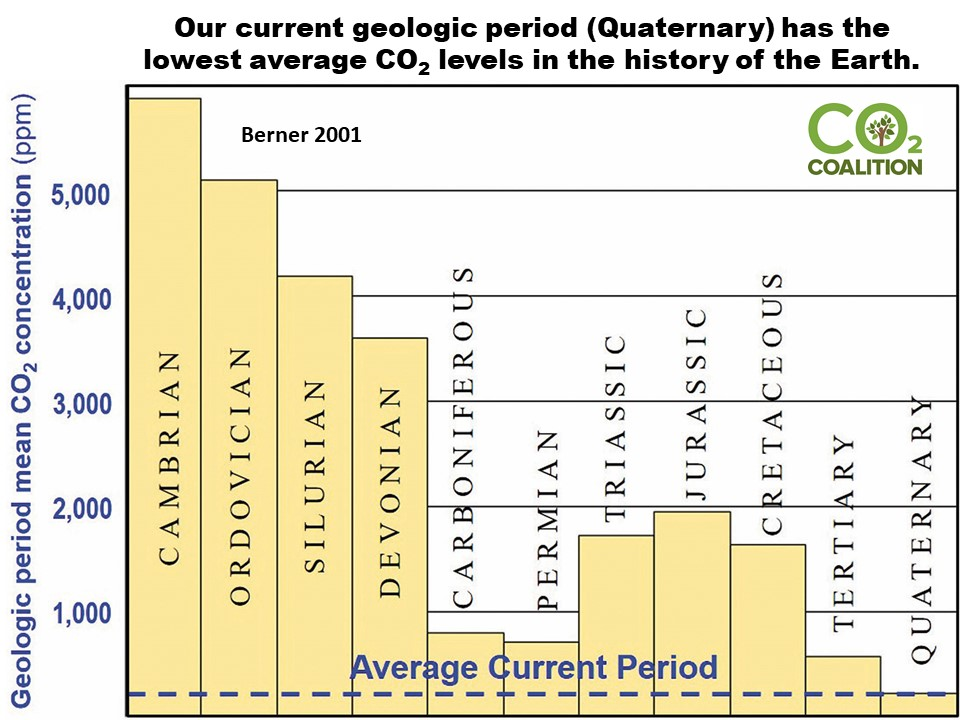
\includegraphics[width=0.8\linewidth]{CO2_evolucao.jpg}
	\caption{Imagem que ilustra a evolução das quantidades de CO2 em ppm durante os períodos da Terra.}
	\label{fig:co2-evolucao}
\end{figure}

A Idade do Gelo, iniciada a aproximadamente 2,6 milhões de anos, registou várias eras glaciais da Terra. Esses períodos de temperaturas glaciais foram interrompidos por períodos interglaciais mais quentes, quando o gelo derreteu e os níveis da água aumentaram. Estima-se que este período tenha terminado há aproximadamente 11.700 anos.

\begin{figure}[H]
	\centering
	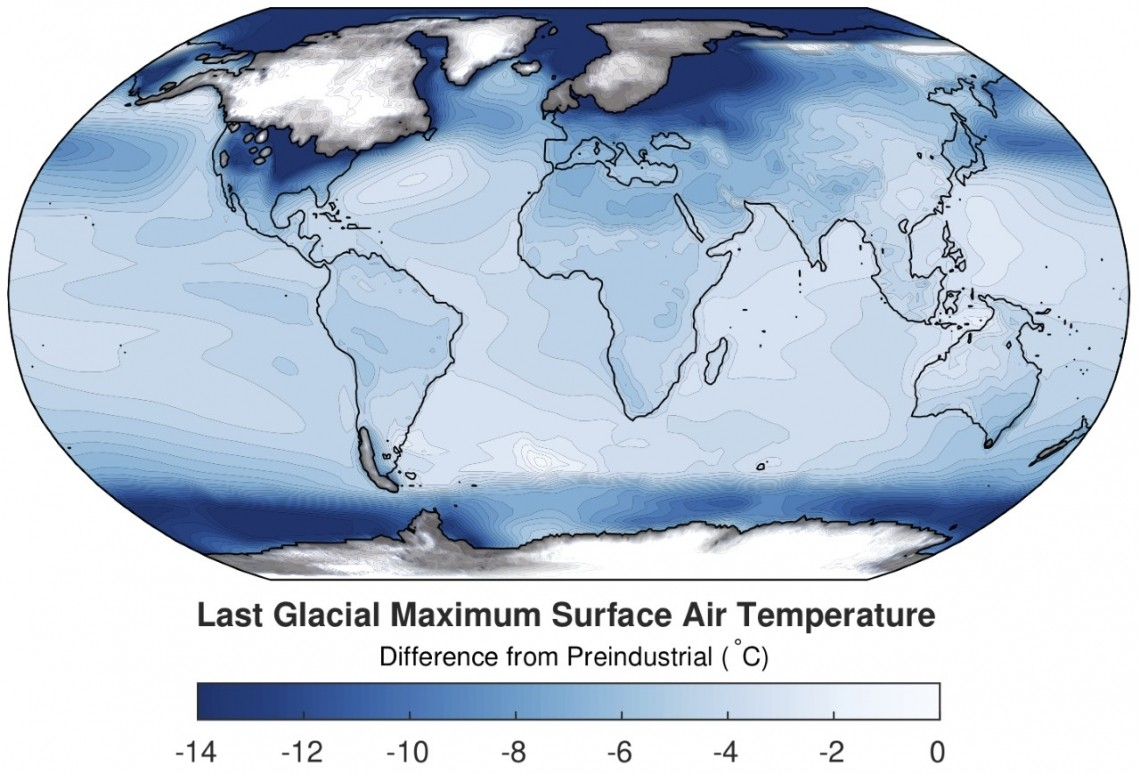
\includegraphics[width=0.8\linewidth]{era_do_gelo.jpg}
	\caption{Imagem ilustrativa quanto à temperatura do ar, à superfície do globo na última glaciação, em graus Celcius.}
	\label{fig:era-do-gelo}
\end{figure}

Compreender a presença histórica das mudanças climáticas na Terra é importante para reconhecer que elas existiam antes dos humanos. Sendo assim, para prever e aliviar os efeitos futuros das \ac{ac}, é necessário sermos portadores do contexto histórico da Terra.

\subsection{Atualidade}
No atual panorama climático, presenciamos mudanças de grande magnitude nas condições atmosféricas globais, refletindo um aumento incontestável das temperaturas em todas as partes do mundo. Este fenómeno, que transcende as flutuações naturais do clima, carrega consigo uma característica marcante: a ação humana emergiu como uma força determinante, traçando um capítulo crucial na história climática de nosso planeta.

Um aumento médio de temperatura emergiu porém este não pode ser meramente atribuído ao ciclo natural das estações. Ao contrário das eras passadas, onde as mudanças climáticas seguiam ritmos geológicos, agora presenciamos um impacto acelerado, impulsionado principalmente por nós (seres humanos). 

\begin{figure}[H]
	\centering
	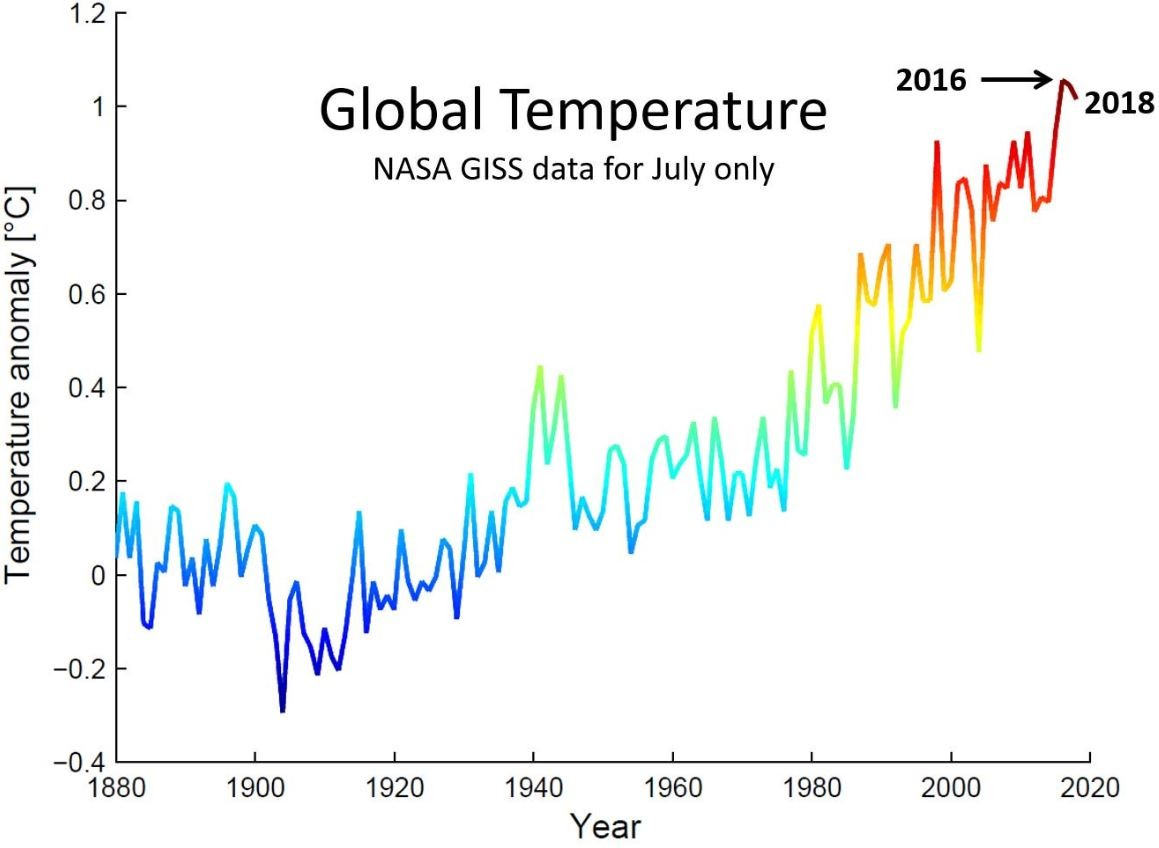
\includegraphics[width=0.8\linewidth]{mudanca_temp.jpg}
	\caption{Gráfico onde são apresentadas as variações da temperatura, em graus Celcius, no mês de julho, entre 1880 e 2020.}
	\label{fig:mudancas_da_temperatura}
\end{figure}

Secas em larga escala e inundações avassaladoras, são muito mais do que desastres ocasionais, são experiências que redefinem a vida de pessoas ao redor do mundo, existem cada vez mais desastre ao redor do globo provocados ou até mesmo agravados pela crise climática. A imprudência climática tem congestionado a vida de todos os seres que habitam este astro, e é possível já evidenciar todos os problemas coadjuvantes aos desastres climáticos.

A ciência encontra-se cada vez mais alarmada com a crise climática, já que as previsões que os mesmos têm concebido ao longo desta ultima década são cada vez mais chocantes. A cada grau de temperatura que é adicionado aos termómetros, ocorrem fenómenos como aumento do nível do mar (provenientes do degelo), a perda de biodiversidade e os riscos à segurança alimentar tornam-se parte intrínseca da narrativa. 

Compreender a natureza humana dessas mudanças não é apenas uma questão científica, mas também um chamado ético e moral para ação. 

Com todos estes problemas à disputa, já foram revelados vários estudos que nos retratam o que o nosso desleixe diário fará ao nosso futuro e ao futuro das nossas gerações, retrataremos isso mais adiante.

\subsection{Futuro}

Quanto ao futuro, apesar de nada ser certo, muitos problemas são previsíveis. Assim sendo, é possível confirmar, através de algumas pesquisas científicas, verificar que toda a problemática atual está diretamente conectada com os distúrbios esperados para o futuro.

A situação encontra-se tão grave que a adoção de políticas ambientais drásticas é atualmente a única maneira de evitar o aumento exponencial da temperatura terrestre:

\begin{figure}[H]
	\centering
	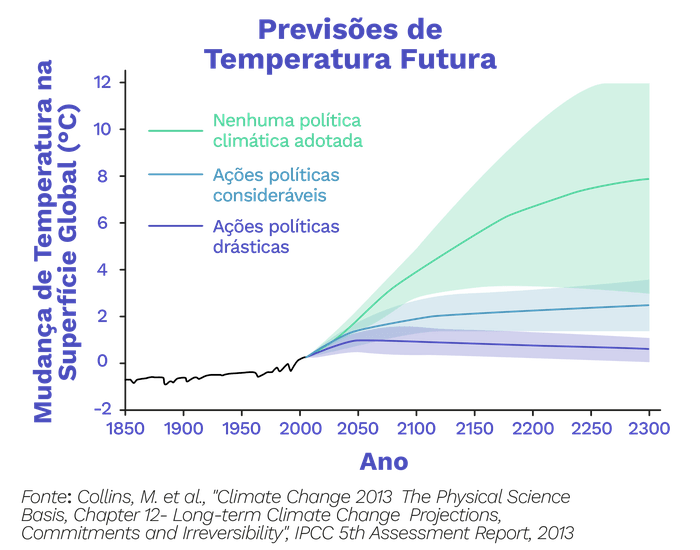
\includegraphics[width=0.8\linewidth]{future_temperature_predictions.png}
	\caption{Gráfico onde são apresentadas as variações da temperatura, em graus Celcius, previstas para o futuro conforme a adoção de políticas relacionadas à sustentabilidade.}
	\label{fig:previsoes_climaticas}
\end{figure}

Para além da temperatura, também está prevista a perda de grande parte da biodiversidade terrestre, apresentando-se como maioria, o número de animais domesticados seguidos da raça humana, entrando a vida selvagem em decadência, (o que provoca o então decréscimo de biodiversidade):

\begin{figure}[H]
	\centering
	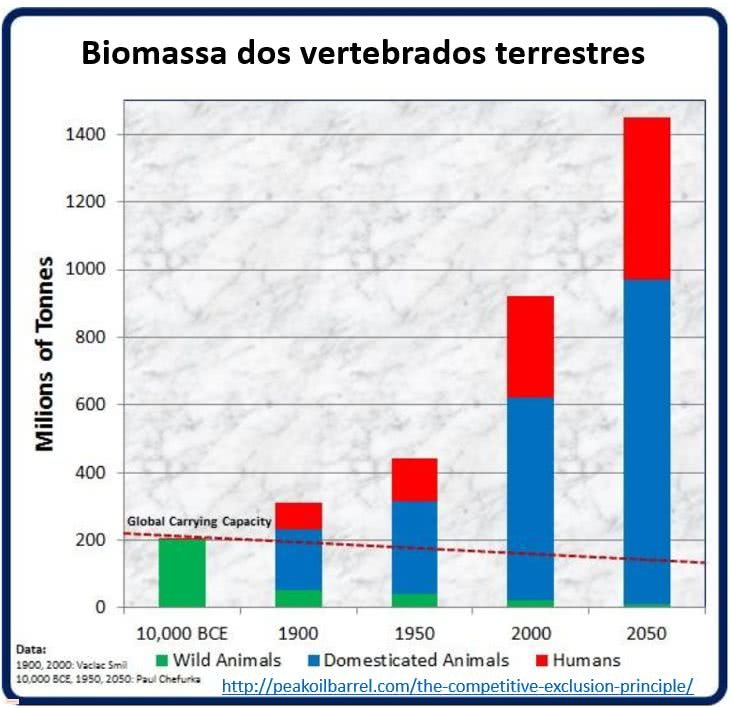
\includegraphics[width=0.8\linewidth]{biodiversidade_queda.jpg}
	\caption{Gráfico que relata ao passar dos anos, o resumo da biodiversidade terrestre, apresentando também uma previsão para 2050.}
	\label{fig:biodiversidade_em_queda}
\end{figure}

Através destes estudos, é possível averiguar que o que o futuro nos espera não é tão risonho quanto o que nós pensávamos, mas como em qualquer dilema, há sempre um principal responsável para que o mesmo se manifeste, ou pelo menos existem sempre contribuinte essenciais para a existência do mesmo.

Abordaremos assim, quem são os principais responsáveis para o aumento das alterações climáticas no capítulo 3.

\chapter{Contribuintes}
\label{chap.resultados}

\section{Mão Humana}
As alterações climáticas são um tema que é cada vez mais abordado, e é inegável a responsabilidade que o Homem tem no estado atual da situação. Este capítulo tem como objetivo explorar como as ações humanas a nível da indústria e do quotidiano do ser humano moldaram o mundo que habitamos hoje.

O grande problema originado das ações do Homem reside na emissão de grandes quantidades de gases de efeito estufa, devido principalmente à queima de combustíveis fósseis, desmatamento e práticas industriais. Estes gases nocivos, entre eles o \ac{co2}, \ac{ch4} e óxidos nitrosos (N2O), são libertados para a atmosfera e absorvem os raios solares e retém o calor fazendo com que seja devolvido para a superfície terrestre só que este fenômeno natural quando ocorrer com grande quantidades desses gases contribuem para o aumento de efeito de estufa, e por consequência para o aquecimento global.

\begin{figure}[H]
	\centering
	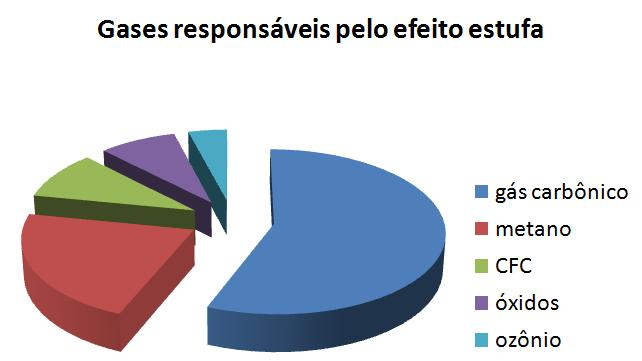
\includegraphics[width=0.8\linewidth]{gasesefeitodeestufa.jpg}
	\caption{Imagem ilustrativa quanto à presença e quantidade de gases efeito de estufa.}
	\label{fig:gases-efeito-de-estufa}
\end{figure}

Estes aumentos devem-se ao crescimento das atividades industriais, à expansão urbana e ao consumo descontrolado dos recursos naturais. E ao invés de se serem todas ações mitigadoras, ocorre desmatamento, para fornecer espaço para agricultura, muitas vezes intensiva, e para o desenvolvimento urbano, isto não apena afeta a habilidade das florestas de absorver \ac{co2} como também liberta grandes quantidades de carbono.

Juntamente com o estilo de vida atual e o aumento da população, as demandas energéticas têm aumentado, o que leva à queima de combustíveis fósseis aumentando ainda mais as emissões de gases de efeito de estufa.

Então, embora as alterações climáticas sejam um fenômeno natural, as ações do Homem têm feito com elas sejam o problema afeta toda a biodiversidade da Terra.


\subsection{Indústrias}
Como destacado anteriormente, as atividades humanas são uma das principais causas das mudanças climáticas que se têm feito sentir nas últimas décadas . Este capítulo irá aprofundar-se no papel que o Homem teve, analisando como as práticas industriais contribuem diretamente para estas modificações no clima da Terra e explorando as consequências para a nossa sobrevivência e para o equilíbrio ecológico.

A extensa queima de combustíveis fósseis destaca-se como a principal culpada nas emissões de carbono industriais. Esse processo liberta grandes quantidades de \ac{co2}, \ac{ch4}, N2O e outros gases de efeito estufa, servindo como um estimulante para o aquecimento global. As consequências dessa atividade vão além do aumento das temperaturas atmosféricas, mas também envolvem impactos adversos em eventos climáticos extremos.

\begin{figure}[H]
	\centering
	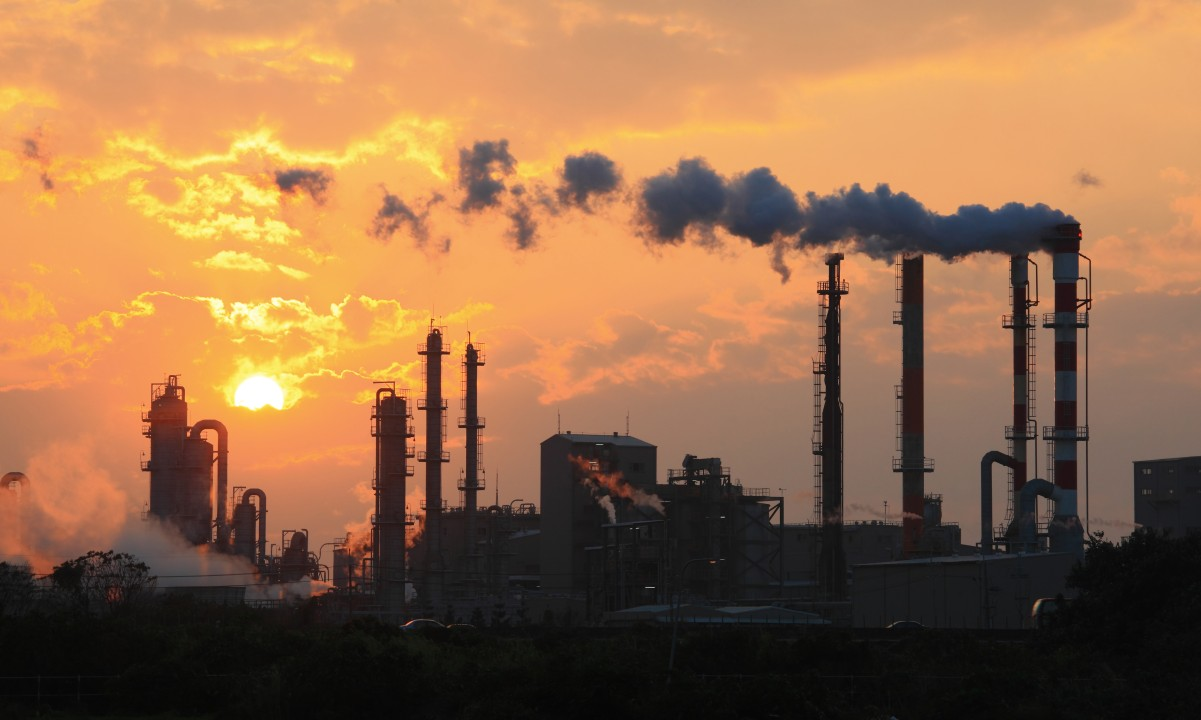
\includegraphics[width=0.8\linewidth]{industriapoluente.jpeg}
	\caption{Imagem onde é possível observar a emissão de gases poluentes na indústria.}
	\label{fig:gases-industria}
\end{figure}

Ao mesmo tempo, a demanda contínua por recursos favorece o desmatamento impulsionado pela indústria, especialmente para a agricultura e para o desenvolvimento urbano, as florestas são assim cada vez mais exploradas, comprometendo a estabilidade dos ecossistemas e libertando o carbono armazenado. Essas emissões aceleradas de gases de efeito estufa contribuem também para \ac{ac}.

As práticas agrícolas modernizadas e a expansão da pecuária são adições cruciais à lista de fontes emissoras, devido à libertação de nitrogênio, \ac{n}, e \ac{ch4} das atividades agrícolas altamente industrializadas. Essas práticas não apenas contaminam o solo e as fontes de água, mas também produzem efeitos duradouros no clima.

Estes são alguns exemplos das consequência que a ação humana provocou para acelerar as \ac{ac}, destaca-se a necessidade urgentes para práticas mais sustentáveis, nos capítulos seguintes serão mostradas estratégias para prevenir futuros danos 

\subsection{Quotidiano}
O \ac{ev} humano surge também como uma força significativa nas \ac{ac}, influenciando o equilíbrio do sistema climático da Terra. As escolhas que tomamos  e as ações que fazemos diariamente têm também um papel crucial neste fenômeno global, como mencionado anteriormente.

O aumento das nossas demandas energéticas, devido ao crescimento populacional global, provocou uma dependência excessiva dos combustíveis fósseis, atividades diária como conduzir e a utilização de ar condicionado, resultam na emissão de grandes quantidades de gases de \ac{ee} que contribuem para o aumento desta.

Além disso, os nossos elevados padrões de consumo resultam numa produção em massa e por consequência num esgotamento dos recursos que a Terra não consegue regenerar à mesma velocidade que os consumimos, e muitas desses processos produtivos libertam grandes quantidades de \ac{co2},  \ac{ch4}, e consomem vastas quantidades de energia, aumentando a pegada de carbono e agravando o problema.

A gestão inadequada de resíduos, caracterizada pelo uso excessivo de materiais não degradáveis, como plástico, e pela eliminação inadequada de resíduos, resulta em poluição que perturba o equilíbrio ecológico da Terra. Estas práticas do nosso \ac{ev} contribuem para os impactos negativos que influenciam as \ac{ac}.

Como se pode ver as escolhas que fazemos diariamente têm sim um impacto nas \ac{ac}, por isso somos todos responsáveis pelo que se tá fazendo sentir.


\chapter{Combate}
\label{chap.analise}

\section{Como minimizar}

Ficou claro que as \ac{ac} são algo que necessita urgentemente de ser minimizado, de modo que como constado anteriormente neste documento, seja possível minimizar a pegada das \ac{ac}.  

\subsection{Adaptação Resiliente}

Adaptação resiliente não se trata de nada mais do que a implementação de medidas a longo prazo de modo a conseguir introduzir uma vida mais sustentável no dia-a-dia das indústrias e até mesmo na nossa própria vida.

Na adaptação resiliente, podemos introduzir medidas como: a promoção de práticas agrícolas sustentáveis, proteção e restauração de ecossistemas naturais e a implementação de políticas que incentivem a redução de emissões de \ac{co2} e gases efeito de estufa.

As práticas agrícolas sustentáveis incluem por exemplo, a promoção da agricultura biológica através da criação de subsídios que apões os cultivadores aderentes a esta prática. A agricultura biológica é um método que facilita a diminuição da poluição, já que não são usados químicos prejudiciais ao ambiente, que possam contribuir de certo modo com as \ac{ac}.

Proteção e restauração de ecossistemas naturais é também essencial, já que estes facilitam e ajudam a reduzir a pegada humana, devolvendo o carácter natural e consequentemente reconstruindo métodos que autrora preveniam também eventos climáticos destrutivos. Entre outras palavras os ecossistemas ajudavam na regulação regular do clima. Tendo em conta estes pontos, a restauração e proteção de habitats pode passar através de várias medidas tais como a criação de zonas protegidas, restauração de habitats degradados e até mesmo a implementação de políticas ambientais que protejam os mesmos.

Finalmente, políticas ambientais que regulem emissões de \ac{co2} e gases efeito de estufa acaba por ser uma das também principais medidas à prevenção das \ac{ac}, uma vez que estes são uns dos principais poluentes e cujo as emissões são mais elevadas.

Em suma, a adaptação resiliente não assume um carácter imediato, e sim uma série de implementações a longo prazo mas que fazem toda a diferença quanto à proteção ambiental, entre outras palavras, não é nada mais que uma mitigação contínua rumo à sustentabilidade.



\section{Como prevenir}

\subsection{Transição para Energia Renovável}

Como falado anteriormente, as emissões de gases poluentes resultam de decisões tanto individuais como industriais, por isso umas das coisas que podem ser feitas para diminuir e até eliminar por completo, em alguns casos, é fazer uma transição global da utilização de energias não renováveis e não sustentáveis para fontes de energia renováveis e mais sustentáveis.

Há várias abordagens que podemos seguir para tornar o nosso \ac{ev} mais “amigo do ambiente”, para poupar energia podemos, por exemplo, apostar em eletrodomésticos de classe A, como microondas e frigoríficos, que consomem menos energia, reduzindo os custos da eletricidade e o desperdícios de recursos naturais, ou instalar em nossas casas paineis solares que alongo prazo reduzem o valor da fatura energética e aumenta a independência energética de nossas casas.

No entanto, estas são formas que nem todas as famílias podem aderir, porém também é possível através de simples ações ser mais sustentável, todos nós podemos apagar as luzes quando saímos de um cômodo, desligar eletrodomésticos da tomada quando não estão em uso, desligar a televisão e optar por lâmpadas Led que poupa 70 \% a 90 \% da energia consumida e optar por ir a pé ou de transportes públicos.

No âmbito empresarial, também podem tomar medidas semelhantes para poupar energia como substituir equipamentos elétricos obsoletos por outros mais eficientes e que consomem menos energia, reaproveitar a energia gerada por processos de produção e realizar relatórios de sustentabilidade que impõem metas e mostram o progresso da poupança.

\begin{figure}[H]
	\centering
	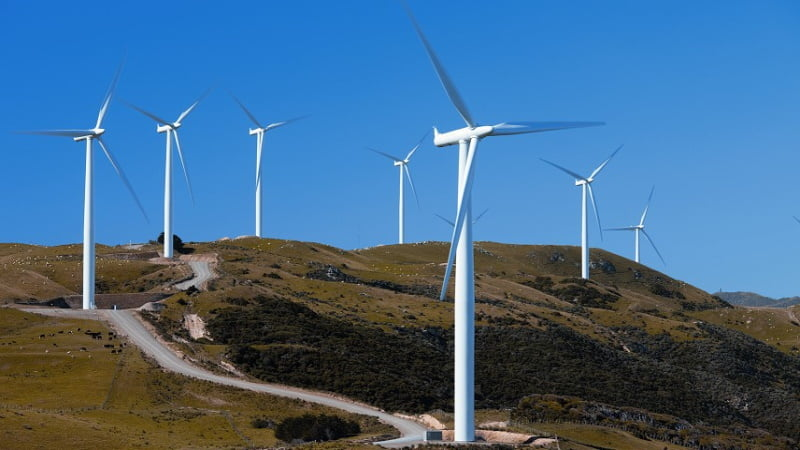
\includegraphics[width=0.8\linewidth]{eolicas.jpg}
	\caption{Imagem representativa de uma energia verde(eólicas).}
	\label{fig:eolicas}
\end{figure}

\subsection{Conservação e Reflorestamento}

Quando não é possível eliminar por completo as fontes de energia não renováveis e não sustentáveis é possível adotar medidas para diminuir os resíduos provenientes destas fontes, por isso adotar boas políticas de gestão de resíduos, tanto a nível pessoal como empresarial, é uma boa forma de prevenir mais as \ac{ac}.

\begin{figure}[H]
	\centering
	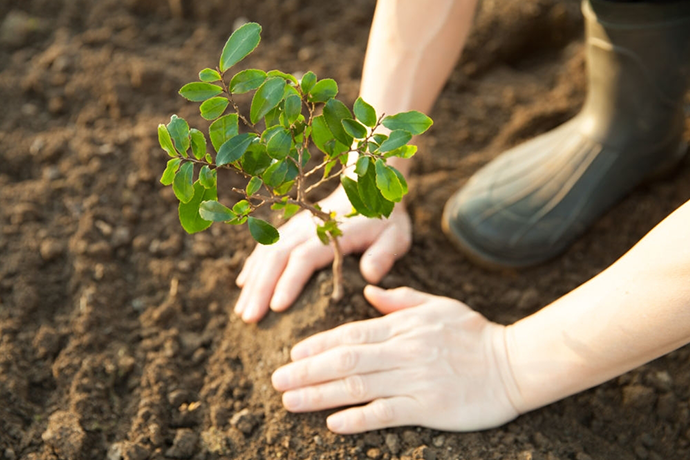
\includegraphics[width=0.8\linewidth]{plantacao.png}
	\caption{Imagem de carácter ilustrativo quanto à reflorestação.}
	\label{fig:plantacao}
\end{figure}

A prática da reciclagem tem se destacado como uma das formas mais populares de contribuir para o ambiente, sendo adotada por várias autarquias do nosso país e cidades por todo o mundo. A política do 3 R’s, “Reduzir, Reutilizar e Reciclar” agora 5 R’s “ Repensar, Recusar, Reduzir, Reutilizar e Reciclar” é uma excelente política a adotar para sermos mais sustentáveis, ela permite uma reflexão dos nossos valores e práticas, com vista ao objetivo de mudarmos os nossos hábitos e reduzir o consumo exagerado e o desperdício focando-nos na reutilização e não apenas na reciclagem. 

\begin{figure}[H]
	\centering
	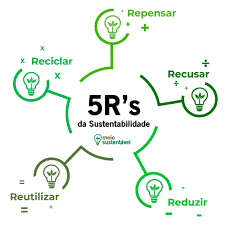
\includegraphics[width=0.8\linewidth]{5r.png}
	\caption{Imagem que ilustra os 5 r's.}
	\label{fig:5rs}
\end{figure}

Esta política pode ser adotada tanto por nós para por exemplo planear refeições para evitar excessos e armazenar alimentos corretamente para prevenir a deterioração, reduzir o consumo de carne, evitar produtos excessivamente embalados e reutilizar garrafas de plástico ou optar por recipientes reutilizáveis como os da \textit{Tupperware}. 

Enquanto que o setor industrial, pode optar por fornecedores que adotem práticas sustentáveis e produtos certificados como sustentáveis, desenvolver e participar de projetos de compensação de carbono, impor normas obrigatórias para a disposição de resíduos que garantam o seu tratamento adequado, evitando a poluição. Agora com as novas tecnologias é possível investir em sistemas que otimizem o processo de produção para diminuir os resíduos e o seu tratamento, reduzindo assim também a necessidade de aterros e instalações de incineração. Já em casos especiais, que envolvem resíduos tóxicos ou perigosos, estes têm de ser tratados na fonte geradora, para reduzir o risco de contaminação no tratamento final. 

Estas são apenas algumas das medidas que podem ser adotadas tanto por nós como pelo setor da indústria para prevenir o aumento da emissão de gases de estufa, mas também para trabalhar em direção a sermos mais sustentáveis.

\subsection{Agricultura Sustentável}

A agricultura sustentável é outra forma de combater as \ac{ac}, que nós e o setor industrial podemos adotar. Com esta prática é possível reduzir os impactos ambientais adversos, contribuir para a manutenção do equilíbrio ecológico e garantir a segurança alimentar futura.

\begin{figure}[H]
	\centering
	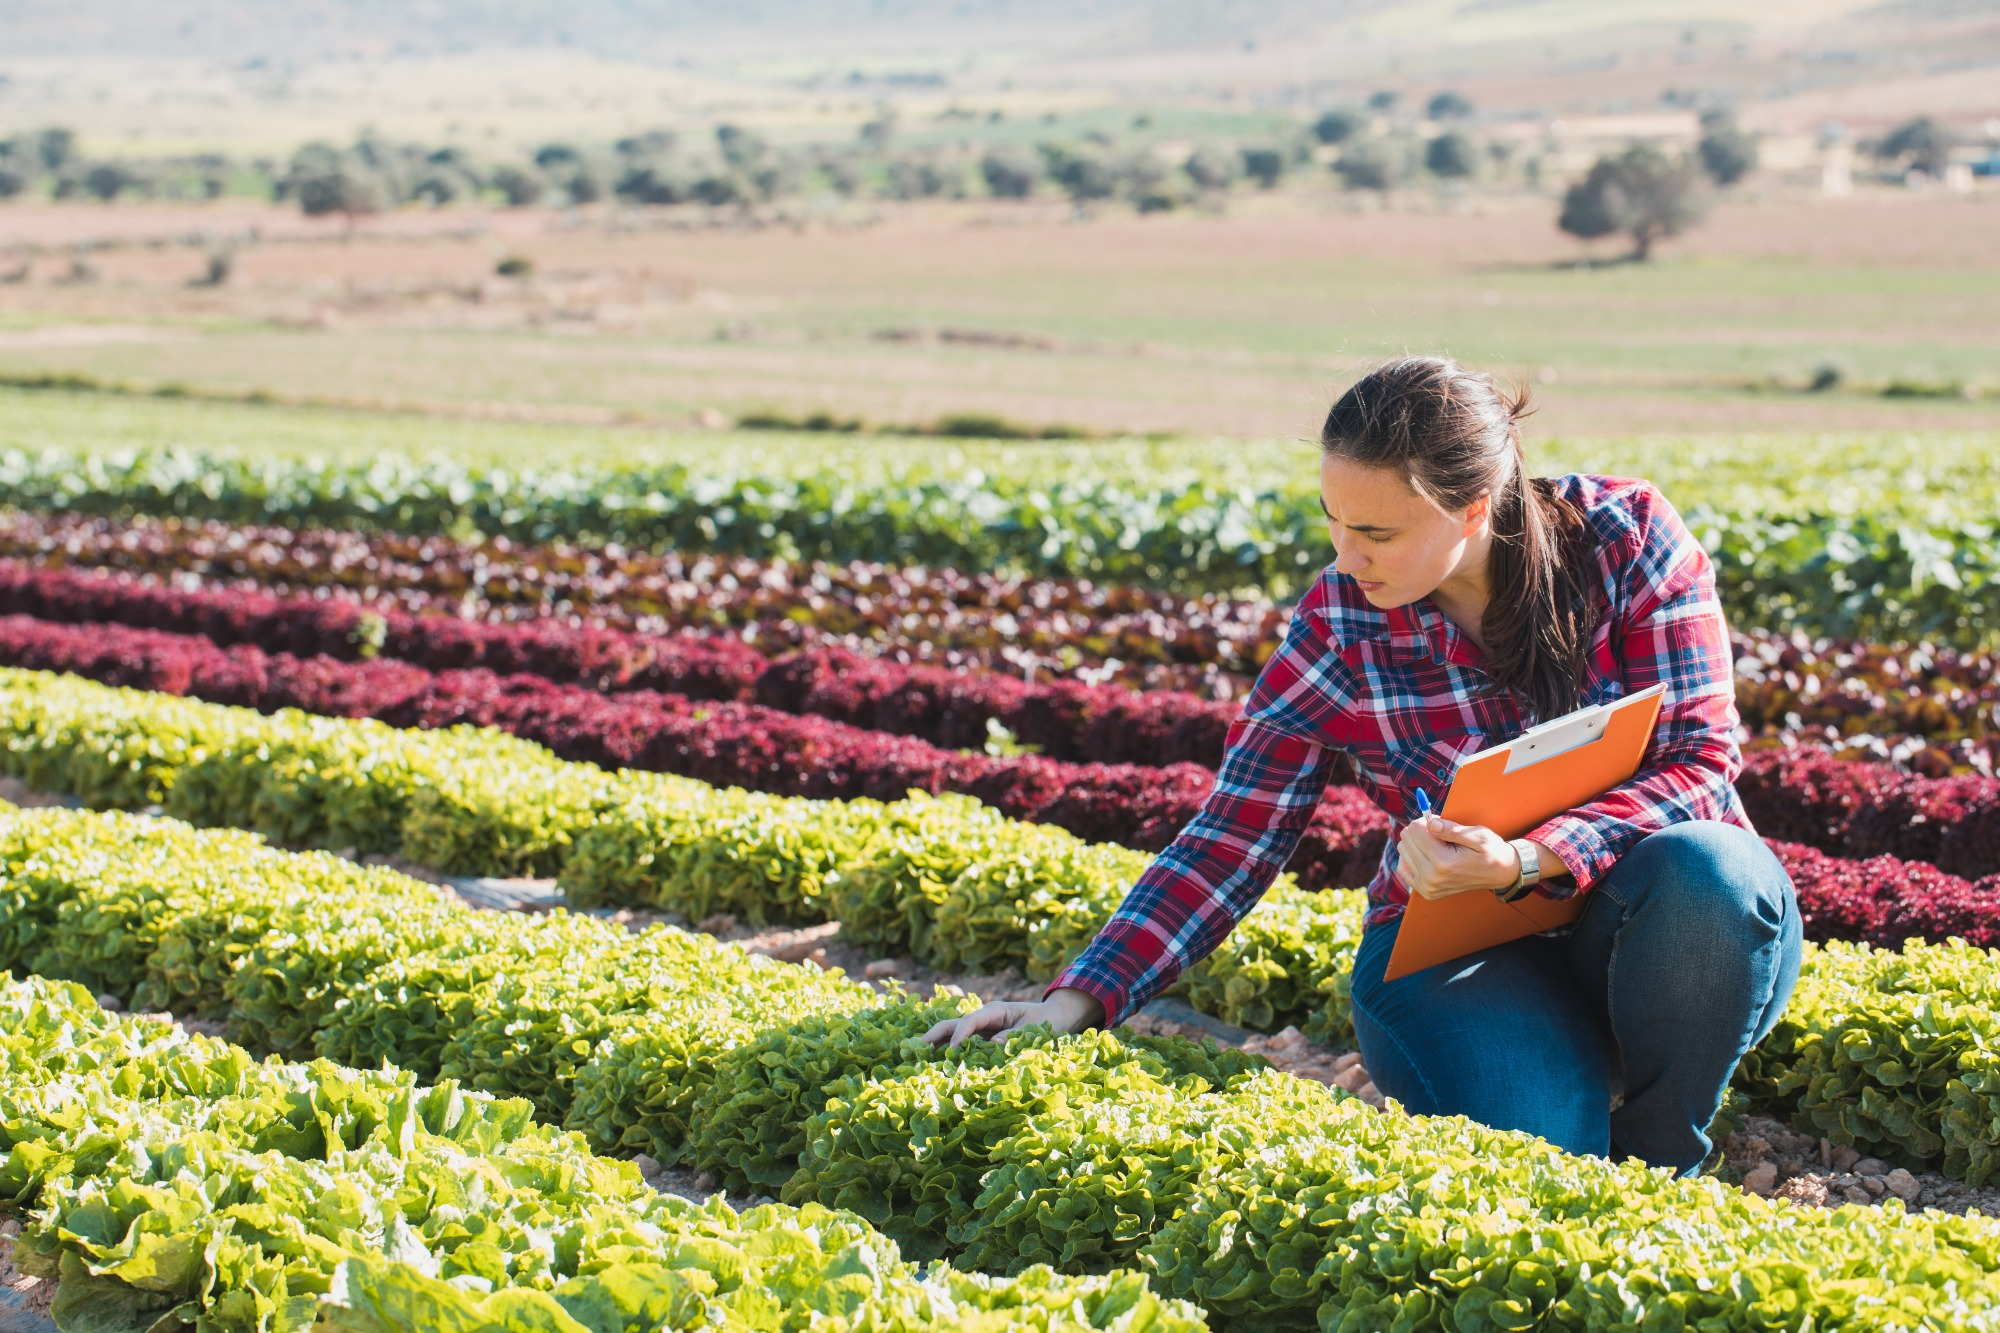
\includegraphics[width=0.8\linewidth]{agriculturasustentavel.jpg}
	\caption{Imagem de carácter ilustrativo quanto à agricultura sustentável.}
	\label{fig:eolicas}
\end{figure}

A nível individual, podemos praticar uma agricultura sustentável tendo por exemplo nas nossas varandas ou quintais uma pequena horta onde podemos plantar alguns alimentos, este hábito permite o cultivo de alimentos livres de contaminação por pesticidas e outros produtos que normalmente contaminam os solos, contribuindo para uma alimentação mais saudável. Também ao consumir produtos de origem local e da temporada reduz as emissões de carbono relacionadas com o transporte de longa distância.

No contexto industrial, podem-se realizar práticas agrícolas sustentáveis como a adoção de sistemas de irrigação que reutilizam a água que proveio da chuva, métodos de fertilização naturais em vez de pesticidas a fim de evitar a contaminação dos solos e de lençóis de água, evitar a monocultura através da rotação de cultivo, protegendo assim a qualidade do solo e a biodiversidade. As novas tecnologias tornam possível fazer uma agricultura mais inteligente e de precisa que permite minimizar os desperdícios de recursos naturais e os impactos ambientais, por exemplo através de sistemas de rega que gastam apenas a quantidade necessária de água.

No que diz respeito à pecuária e pesca mais sustentável, a adoção de práticas de pastoreio rotativo evita a degradação do solo e o desenvolvimento excessivo da terra, alterar a rações dos animais pode reduzir a emissão de gases do efeito de estufa provenientes da digestão dos animais, levando à redução da pegada de carbono. Medidas de fechamento sazonal das zonas de pesca alinhadas com os períodos de desova ajudar a manter o equilíbrio no ecossistema aquático

Esta prática de agricultura sustentável não só contribui para prevenir as \ac{ac} como também contribui para a conservação dos solos, da água e dos ecossistemas.

\chapter{Conclusões}
\label{chap.conclusao}
Ao decorrer da tese, foram abordadas as várias facetas das \ac{ac}, desde a sua origem no passado até mesmo ás previsões quanto ao futuro das mesmas.
Aprofundámos a nossa compreensão quanto aos fatores contribuintes, destacando a mão humana como principal fator para o aumento a larga escala das mesmas. Exploramos os caminhos para minimizar e prevenir as \ac{ac} e também as oportunidades e responsabilidades que o globo tem.

Os resultados desta pesquisa contribuiram para percebermos que as \ac{ac} ultrapassam barreiras geográficas e exigem uma elevada preocupação humanitária, ou seja, são necessárias medidas coerentes para enfrentar esta problemática.

Em última instância, para além de destacarmos a urgência climática, temos de enfatizar a necessidade de contribuirmos responsavelmente de maneira autónoma, rumo a um futuro mais sustentável. Assim, espera-se que estas conclusões sejam utilizadas como um apelo à consciencialização, mas também ação, de modo a irmos rumo a um futuro mais sustentável. 





\chapter*{Contribuições dos autores}
Este trabalho envolveu muito esforço de ambas as partes, tendo a \ac{cr} tratado essencialmente do capítulo 2 e subcapítulo 4.1 e a \ac{rg} tratado do capítulo 3 e subcapítulo 4.2.
Ambos os autores analisaram de maneira crítica e construtiva o trabalho, procedendo também à revisão do mesmo.
Assim sendo, decidimos que seria mais que justo atribuir a ambas a mesma percentagem de contribuição. 



\vspace{10pt}
\textbf{Indicar a percentagem de contribuição de cada autor.}\\

\autores : 50\%, 50\%\\

%%%%%%%%%%%%%%%%%%%%%%%%%%%%%%%%%
\chapter*{Acrónimos}
\begin{acronym}
	\acro{ua}[UA]{Universidade de Aveiro}
	\acro{leci}[LECI]{Licenciatura em Engenharia de Computadores e Informática}
	\acro{glisc}[GLISC]{Grey Literature International Steering Committee}
	\acro{cr}[CR]{Catarina Monteiro Rabaça}
	\acro{rg}[RG]{Rita Pipa Godinho}
	\acro{ac}[AC]{Alterações Climáticas}
	\acro{co2}[CO2]{Dióxido de carbono}
	\acro{ch4}[CH4]{Metano}
	\acro{n}[N]{Nitrogénio}
	\acro{ev}[EV]{Estilo de vida}
	\acro{ee}[EE]{Efeito de Estufa}
	
\end{acronym}

%%%%%%%%%%%%%%%%%%%%%%%%%%%%%%%%%
\printbibliography

\end{document}
